%% Copyright (c) 2015-2019, RTE (http://www.rte-france.com)
%% See AUTHORS.txt
%% All rights reserved.
%% This Source Code Form is subject to the terms of the Mozilla Public
%% License, v. 2.0. If a copy of the MPL was not distributed with this
%% file, you can obtain one at http://mozilla.org/MPL/2.0/.
%% SPDX-License-Identifier: MPL-2.0
%%
%% This file is part of Dynawo, an hybrid C++/Modelica open source time domain simulation tool for power systems.

\documentclass[a4paper, 12pt]{report}

%% Except where otherwise noted, content in this documentation is Copyright (c)
%% 2015-2019, RTE (http://www.rte-france.com) and licensed under a
%% CC-BY-4.0 (https://creativecommons.org/licenses/by/4.0/)
%% license. All rights reserved.

% Latin Modern fam­ily of fonts
\usepackage{lmodern}

\usepackage[english]{babel}

% specify encoding
\usepackage[utf8]{inputenc} % input
\usepackage[T1]{fontenc} % output

% Document structure setup
\usepackage{titlesec} % To change chapter format
\setcounter{tocdepth}{3} % Add subsubsection in Content
\setcounter{secnumdepth}{3} % Add numbering for subsubsection
\setlength{\parindent}{0pt} % No paragraph indentation

% Change title format for chapter
\titleformat{\chapter}{\Huge\bf}{\thechapter}{20pt}{\Huge\bf}

% To add links on page number in Content and hide red rectangle on links
\usepackage[hidelinks, linktoc=all]{hyperref}
\usepackage[nottoc]{tocbibind}  % To add biblio in table of content
\usepackage{textcomp} % For single quote
\usepackage{url} % Allow linebreaks in \url command
\usepackage{listings} % To add code samples

% Default listings parameters
\lstset
{
  aboveskip={1\baselineskip}, % a bit of space above
  backgroundcolor=\color{shadecolor}, % choose the background color
  basicstyle={\ttfamily\footnotesize}, % use font and smaller size \small \footnotesize
  breakatwhitespace=true, % sets if automatic breaks should only happen at whitespace
  breaklines=true, % sets automatic line breaking
  columns=fixed, % nice spacing -> fixed / flexible
  mathescape=false, % escape to latex false
  numbers=left, % where to put the line-numbers
  numberstyle=\tiny\color{gray}, % the style that is used for the line-numbers
  showstringspaces=false, % do not emphasize spaces in strings
  tabsize=4, % number of spaces of a TAB
  texcl=false, % activates or deactivates LaTeX comment lines
  upquote=true % upright quotes
}

% Avoid numbering starting at each chapter for figures
\usepackage{chngcntr}
\counterwithout{figure}{chapter}

\usepackage{tikz} % macro pack­age for cre­at­ing graph­ics
\usepackage{pgfplots} % draws func­tion plots (based on pgf/tikz)

\usepackage{algorithm} % Add algorithms
\usepackage[noend]{algpseudocode} %  all end ... lines are omitted in algos

\usepackage{amsmath} % Add math­e­mat­i­cal fea­tures
\usepackage{schemabloc} % Add block diagram library (french one)

\usepackage{adjustbox} % Add box for flowchart

\usepackage{booktabs} % for toprule and midrule in tables

\usepackage{tabularx}

\usepackage[nolist]{acronym} % don’t write the list of acronyms.
% Acronyms list
\begin{acronym}
\acro{BDF}{Backward Differentiation Formula}
\acro{BE}{Backward Euler}
\acro{DAE}{Differential Algebraic Equations}
\acro{IDA}{Implicit Differential-Algebraic solver}
\acro{LLNL}{Lawrence Livermore National Lab}
\acro{KINSOL}{Krylov Inexact Newton SOLver}
\acro{NR}{Newton-Raphson}
\acro{PLL}{Phase-Locked Loop}
\acro{SVC}{Static Var Compensator}
\acro{SUNDIALS}{SUite of Nonlinear and DIfferential/ALgebraic equation Solvers}
\acro{WECC}{Western Electricity Coordinating Council}
\end{acronym}

% Syntax highlight
%% Except where otherwise noted, content in this documentation is Copyright (c)
%% 2015-2019, RTE (http://www.rte-france.com) and licensed under a
%% CC-BY-4.0 (https://creativecommons.org/licenses/by/4.0/)
%% license. All rights reserved.

\usepackage{color}

\definecolor{blue}{rgb}{0,0,1}
\definecolor{lightblue}{rgb}{.3,.5,1}
\definecolor{darkblue}{rgb}{0,0,.4}
\definecolor{red}{rgb}{1,0,0}
\definecolor{darkred}{rgb}{.56,0,0}
\definecolor{pink}{rgb}{.933,0,.933}
\definecolor{purple}{rgb}{0.58,0,0.82}
\definecolor{green}{rgb}{0.133,0.545,0.133}
\definecolor{darkgreen}{rgb}{0,.4,0}
\definecolor{gray}{rgb}{.3,.3,.3}
\definecolor{darkgray}{rgb}{.2,.2,.2}
\definecolor{shadecolor}{gray}{0.925}

% **********************************************************************************
% Syntax : Bash (bash)
% **********************************************************************************

\lstdefinelanguage{bash}
{
  keywordstyle=\color{blue},
  morekeywords={
    cd,
    export,
    source},
  numbers=none,
  deletekeywords={jobs}
}

% **********************************************************************************
% Syntax : XML
% **********************************************************************************

\lstdefinelanguage{XML}
{
  morestring=[s][\color{purple}]{"}{"},
  morecomment=[s][\color{green}]{<?}{?>},
  morecomment=[s][\color{green}]{<!--}{-->},
  stringstyle=\color{black},
  identifierstyle=\color{blue},
  keywordstyle=\color{red},
  morekeywords={
    xmlns,
    xsi,
    noNamespaceSchemaLocation,
    type,
    source,
    target,
    version,
    tool,
    transRef,
    roleRef,
    objective,
    eventually}
}

% **********************************************************************************
% Syntax : Modelica (modelica)
% **********************************************************************************
\lstdefinelanguage{Modelica}{
  alsoletter={...},
  morekeywords=[1]{ % types
      Boolean,
      Integer,
      Real},
  keywordstyle=[1]\color{red},
  morekeywords=[2]{ % keywords
    algorithm,
    and,
    annotation,
    assert,
    block,
    class,
    connector,
    constant,
    discrete,
    else,
    elseif,
    elsewhen,
    end,
    equation,
    exit,
    extends,
    external,
    false,
    final,
    flow,
    for,
    function,
    if,
    in,
    inner,
    input,
    import,
    loop,
    model,
    nondiscrete,
    not,
    or,
    outer,
    output,
    package,
    parameter,
    public,
    protected,
    record,
    redeclare,
    replaceable,
    return,
    size,
    terminate,
    then,
    true,
    type,
    when,
    while},
  keywordstyle=[2]\color{darkred},
  morekeywords=[3]{ % functions
    abs,
    acos,
    asin,
    atan,
    atan2,
    Complex,
    connect,
    conj,
    cos,
    cosh,
    cross,
    der,
    edge,
    exp,
    fromPolar,
    imag,
    noEvent,
    pre,
    sign,
    sin,
    sinh,
    sqrt,
    tan,
    tanh},
  keywordstyle=[3]\color{blue},
  morecomment=[l][\color{green}]{//}, % comments
  morecomment=[s][\color{green}]{/*}{*/}, % comments
  morestring=[b][\color{pink}]{'}, % strings
  morestring=[b][\color{pink}]{"}, % strings
}


\usepackage{xspace} % Define typography
\usepackage{dirtree}
\newcommand{\Dynawo}[0]{Dyna$\omega$o\xspace}


\begin{document}

\chapter{Static Var Compensator - Infinite Bus}

The \{Static Var Compensator - Infinite Bus\} test case is a simplified system used to illustrate the behaviour of the Static Var Compensator model present in the \Dynawo library on events such as a voltage reference change, a load variation or a node fault.\\

The test case exists in \Dynawo and OpenModelica format. For the first one, the test case files are in the non-regression tests directory. For the second one, they are in the Examples section of the \Dynawo Modelica library.

\section{Test case description}

The following test case consists of a static var compensator connected to an infinite bus through a line as presented in Figure ~\ref{TestCase}.

\begin{figure}[H]
\centering
\def\factor{0.4}
\begin{tikzpicture}[every node/.style={inner sep=0,outer sep=0}]
% Infinite bus
\path (0,0)  pic[scale=0.4,local bounding box=bus] {infinite bus};
% Generator
\path (8,0) pic[scale=0.2,local bounding box=svarc] {SVarC};
% Line 1
\draw (bus.east) -- (svarc.west);
% Bus inf
\draw (bus.east) ++ (0,0.6) --++ (0,-1.2);
% Bus tfo 2
\draw (svarc.west) ++ (-1,0.6) --++ (0,-1.2);
\end{tikzpicture}
\caption{Static Var Compensator - Infinite Bus system representation}
\label{TestCase}
\end{figure}

\subsection{Initial Conditions}

The static var compensator base voltage is $UNom = 225 kV$.

The static var compensator apparent power is $SNom = 250 MVA$.

The line parameters in per unit on 100 MVA base are:
\begin{center}
\begin{tabular}{l|l}
   $R = 0 pu$ & $X = 0.027654 pu$  \\
\end{tabular}
\end{center}

At $t=0s$, the static var compensator injects 0 MW and 0 Mvar, so its terminal voltage is 1 pu

\subsection{Model}

The static var compensator is modeled thanks to a B-G injector controlled by a control model.

\subsubsection{B-G Injector}
The static var compensator can be seen as a variable admittance and is thus modelled thanks to a B-G injector.\\

The B-G injector is a current injector. Its injected complex current i is computed thanks to the susceptance B, the conductance G and the complex voltage at its terminal u with the following equation:
\[
\begin{aligned}
& i = Y*u \\
\end{aligned}
\]
where Y is the complex admittance defined as:
\[
\begin{aligned}
& Y = G + j*B \\
\end{aligned}
\]
The susceptance B and the conductance G are given by the control model.

\subsubsection{Control model}

The control model is all perunited in the SNom base.\\

The conductance represents the active power losses of the static var compensator. Here we neglect the losses so $G_{Pu} = 0$.\\

The susceptance represents the reactive power contribution of the static var compensator. The susceptance computation in per unit depends on the static var compensator regulation mode:

\begin{itemize}
\item if mode = OFF, $B_{Pu} = 0$. The static var compensator doesn't inject reactive power;
\item if mode = STANDBY, $B_{Pu} = BShunt_{Pu}$.
The static var compensator behaves as a  capacitor;
\item if mode = RUNNING\_V, $B_{Pu} = BVar_{Pu} + BShunt_{Pu}$. The susceptance in per unit $B_{Pu}$ is composed of a variable susceptance $BVar_{Pu}$ and a fixed susceptance $BShunt_{Pu}$. The fixed susceptance $BShunt_{Pu}$ represents the susceptance in standby mode, and the variable susceptance $BVar_{Pu}$ represents the equivalent variable susceptance generated by the static var compensator power electronics and enabling to control the voltage.
\end{itemize}

The variable susceptance is computed as depicted in Figure ~\ref{Regulation}:
\begin{figure}[H]
\centering
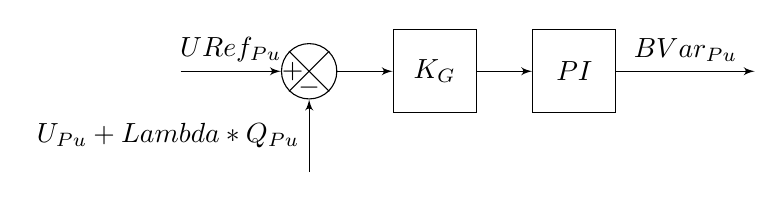
\begin{tikzpicture}
\sbEntree{E}
\sbCompSum[5]{err}{E}{}{-}{+}{}
\sbRelier[$URef_{Pu}$]{E}{err}
\sbDecaleNoeudy[4]{err}{Us}
\sbRelier[$ U_{Pu} + Lambda*Q_{Pu}$]{Us}{err}
\sbBloc{Gain}{$K_G$}{err}
\sbRelier{err}{Gain}
\sbBlocL{PI}{$PI$}{Gain}
\sbSortie[5]{S}{PI}
\sbRelier[$BVar_{Pu}$]{PI}{S}
\end{tikzpicture}
\caption{Variable susceptance regulation}
\label{Regulation}
\end{figure}

The susceptance regulation is based on a PI controller implementing the following regulation law:
\[
\begin{aligned}
& URef_{Pu} = U_{Pu} + Lambda*Q_{Pu}\\
\end{aligned}
\]

In case the voltage is too low, as during a severe three phase fault, the static var compensator can be blocked. In that case the susceptance is set to zero.\\

The variable susceptance $BVar_{Pu}$ is limited thanks to limitations taking into account static susceptance limits and variable current limits.

\subsection{Scenarios}
The simulated scenarios are :
\begin{itemize}
\item a step on the reference voltage;
\item a small reactive load variation;
\item a large reactive load variation;
\item a manual mode change;
\item an impedant three-phase fault;
\end{itemize}

\subsection{Solver}
The solver used is the variable time step solver IDA with the following parameters:
\begin{center}
\begin{tabular}{l|l|l}
   $Order$=2 & $Accuracy_{Rel}$=10e-4 & $Accuracy_{Abs}$=10e-4 \\
\end{tabular}
\end{center}

\newpage
\section{Results}

\subsection{Step on the reference voltage}

The SVarC is initially running. A step on URef from 225 kV to 230kV is realised at $t=1s$.

\begin{figure}[H]
\subfigure[Voltage (kV)]
{%
  \begin{tikzpicture}
    \begin{axis}[height = 1.7in]
       \addplot[color=blue!50]
       table[x=time,y expr=\thisrow{SVarC_SVarC_injector_UPu}*225]
       {../SVarC_1_StepURef/reference/outputs/curves/curves.csv};
    \end{axis}
  \end{tikzpicture}
}
\subfigure[Reactive power (Mvar)]
{%
  \begin{tikzpicture}
    \begin{axis}[height = 1.7in]
       \addplot[color=blue!50]
       table[x=time,y expr=\thisrow{SVarC_SVarC_injector_QInjPu}*100]
       {../SVarC_1_StepURef/reference/outputs/curves/curves.csv};
    \end{axis}
  \end{tikzpicture}
}
\subfigure[Susceptance (pu)]
{%
  \begin{tikzpicture}
    \begin{axis}[height = 1.7in]
        \addplot[color=blue!50]
       table[x=time,y expr=\thisrow{SVarC_SVarC_injector_BPu}]
       {../SVarC_1_StepURef/reference/outputs/curves/curves.csv};
    \end{axis}
  \end{tikzpicture}
}
\caption{Step on the reference voltage}
\end{figure}

At $t=1s$, the SVarC starts providing reactive power to follow the voltage reference change.

\newpage
\subsection{Reactive load variation}

The SVarC is initially in the standby mode. A reactive load variation of Q=150 Mvar is realised at $t=1s$.

\begin{figure}[H]
\subfigure[Voltage (kV)]
{%
  \begin{tikzpicture}
    \begin{axis}[height = 1.7in]
        \addplot[color=blue!50]
       table[x=time,y expr=\thisrow{SVarC_SVarC_injector_UPu}*225]
       {../SVarC_2_LoadVarQ/reference/outputs/curves/curves.csv};
    \end{axis}
  \end{tikzpicture}
}
\subfigure[Reactive power (Mvar)]
{%
  \begin{tikzpicture}
    \begin{axis}[height = 1.7in]
        \addplot[color=blue!50]
       table[x=time,y expr=\thisrow{SVarC_SVarC_injector_QInjPu}*100]
       {../SVarC_2_LoadVarQ/reference/outputs/curves/curves.csv};
    \end{axis}
  \end{tikzpicture}
}
\subfigure[Susceptance (pu)]
{%
  \begin{tikzpicture}
    \begin{axis}[height = 1.7in]
        \addplot[color=blue!50]
       table[x=time,y expr=\thisrow{SVarC_SVarC_injector_BPu}]
       {../SVarC_2_LoadVarQ/reference/outputs/curves/curves.csv};
    \end{axis}
  \end{tikzpicture}
}
\caption{Small reactive load variation}
\end{figure}

At $t=1s$, the voltage suddenly drops due to the load variation and crosses UthresholdDown (218 kV). As a consequence, the SVarC switches to running mode and starts providing reactive power to support the voltage.

\newpage
\subsection{Large reactive load variation}

The SVarC is initially in the standby mode. A large reactive load variation of Q=300 Mvar is realised at $t=1s$.

\begin{figure}[H]
\subfigure[Voltage (kV)]
{%
  \begin{tikzpicture}
    \begin{axis}[height = 1.7in]
       \addplot[color=blue!50]
       table[x=time,y expr=\thisrow{SVarC_SVarC_injector_UPu}*225]
       {../SVarC_3_LoadVarQLarge/reference/outputs/curves/curves.csv};
    \end{axis}
  \end{tikzpicture}
}
\subfigure[Reactive power (Mvar)]
{%
  \begin{tikzpicture}
    \begin{axis}[height = 1.7in]
        \addplot[color=blue!50]
       table[x=time,y expr=\thisrow{SVarC_SVarC_injector_QInjPu}*100]
       {../SVarC_3_LoadVarQLarge/reference/outputs/curves/curves.csv};
    \end{axis}
  \end{tikzpicture}
}
\subfigure[Current (pu)]
{%
  \begin{tikzpicture}
    \begin{axis}[height = 1.7in]
       \addplot[color=blue!50]
       table[x=time,y expr=\thisrow{SVarC_SVarC_regulation_IPu}]
       {../SVarC_3_LoadVarQLarge/reference/outputs/curves/curves.csv};
       \addplot[color=red!50]
       table[x=time,y expr=\thisrow{SVarC_SVarC_regulation_IMaxPu}]
       {../SVarC_3_LoadVarQLarge/reference/outputs/curves/curves.csv};
        \legend{$IPu$, $IMinPu$}
    \end{axis}
  \end{tikzpicture}
}
\caption{Large reactive load variation}
\end{figure}

At $t=1s$, the voltage suddenly drops due to the load variation and crosses UthresholdDown (218 kV). As a consequence, the SVarC switches to running mode and starts providing reactive power to support the voltage. The provided current reaches its limitation and the current limitor is activated in order to bring the current back to an acceptable value.

\newpage
\subsection{Manual mode change}

The SVarC is initially running. A step on URef from 225 kV to 230kV is realised at t=1s. \\

The static var compensator is then turned in manual mode from $t=0.5s$ to $t=5s$,  switched off from $t=3s$ to $t=4s$ and switched back on from $t=4s$. \\

The user variables enabling to simulate this scenario are $selectModeAuto$ and $setMode$.

\begin{figure}[H]
\subfigure[Variable indicating whether the SVarC mode can be changed manually]
{
  \begin{tikzpicture}
    \begin{axis}[height = 1.7in]
       \addplot[color=blue!50]
       table[x=time,y expr=\thisrow{SVarC_SVarC_modeHandling_selectModeAuto}]
       {../SVarC_4_ModeChange/reference/outputs/curves/curves.csv};
        \legend{$selectModeAuto$}
    \end{axis}
  \end{tikzpicture}
}
\subfigure [Variable indicating the desired mode]
{
  \begin{tikzpicture}
    \begin{axis}[height = 1.7in]
       \addplot[color=blue!50]
       table[x=time,y expr=\thisrow{SVarC_SVarC_modeHandling_setModeManual}]
       {../SVarC_4_ModeChange/reference/outputs/curves/curves.csv};
        \legend{$setMode$}
    \end{axis}
  \end{tikzpicture}

}
\end{figure}

The correlation table between the values of $setMode$ and $mode$ is:
\begin{center}
\begin{tabular}{|c|c|}
  \hline
  setMode & mode \\
  \hline
  1 & OFF \\
  \hline
  2 & STANDBY \\
  \hline
  3 & RUNNING-V\\
  \hline
\end{tabular}
\end{center}

\begin{figure}[H]
\subfigure [Current mode of the static var compensator]
{
  \begin{tikzpicture}
    \begin{axis}[height = 1.7in]
       \addplot[color=blue!50]
       table[x=time,y expr=\thisrow{SVarC_SVarC_modeHandling_mode}]
       {../SVarC_4_ModeChange/reference/outputs/curves/curves.csv};
        \legend{$Mode$}
    \end{axis}
  \end{tikzpicture}
}
\subfigure [Voltage (kV)]
{
  \begin{tikzpicture}
    \begin{axis}[height = 1.7in]
       \addplot[color=blue!50]
       table[x=time,y expr=\thisrow{SVarC_SVarC_injector_UPu}*225]
       {../SVarC_4_ModeChange/reference/outputs/curves/curves.csv};
        \legend{$Voltage$}
    \end{axis}
  \end{tikzpicture}
}
\subfigure [Susceptance (pu)]
{
  \begin{tikzpicture}
    \begin{axis}[height = 1.7in]
       \addplot[color=blue!50]
       table[x=time,y expr=\thisrow{SVarC_SVarC_injector_BPu}]
       {../SVarC_4_ModeChange/reference/outputs/curves/curves.csv};
        \legend{$Susceptance$}
    \end{axis}
  \end{tikzpicture}
}
\end{figure}

At $t=1s$, the SVarC starts providing reactive power to follow the voltage reference change. \\

From $t=3s$ to $t=4s$, the SVarC is switched off: its mode is "OFF", its susceptance is zero and no reactive power is injected to the grid.\\

From $t=4s$ on, the SVarC is back in running mode and starts regulating the voltage again.


\newpage
\subsection{Impedent three-phase fault}

The SVarC is initially running. An impedent 100ms three-phase short circuit is simulated from $t=1s$ to $t=1,1s$.

\begin{figure}[H]
\subfigure[Voltage (kV)]
{%
  \begin{tikzpicture}
    \begin{axis}[height = 1.6in]
        \addplot[color=blue!50]
       table[x=time,y expr=\thisrow{SVarC_SVarC_injector_UPu}*225]
       {../SVarC_5_FaultImp/reference/outputs/curves/curves.csv};
    \end{axis}
  \end{tikzpicture}
}
\subfigure[Reactive power (Mvar)]
{%
  \begin{tikzpicture}
    \begin{axis}[height = 1.6in]
        \addplot[color=blue!50]
       table[x=time,y expr=\thisrow{SVarC_SVarC_injector_QInjPu}*100]
       {../SVarC_5_FaultImp/reference/outputs/curves/curves.csv};
    \end{axis}
  \end{tikzpicture}
}
\subfigure[Susceptance (pu)]
{%
  \begin{tikzpicture}
    \begin{axis}[height = 1.6in]
        \addplot[color=blue!50]
       table[x=time,y expr=\thisrow{SVarC_SVarC_injector_BPu}]
       {../SVarC_5_FaultImp/reference/outputs/curves/curves.csv};
       \addplot[color=red!50]
       table[x=time,y expr=\thisrow{SVarC_SVarC_regulation_limitations_BVarMaxPu}]
       {../SVarC_5_FaultImp/reference/outputs/curves/curves.csv};
        \legend{$BPu$, $BMaxPu$}
    \end{axis}
  \end{tikzpicture}
}
\caption{Impedant three-phase fault}
\end{figure}

From $t=1s$ to $t=1.1s$ (during the fault), the SVarC provides the maximum available reactive power in order to support the voltage. Indeed, we observe that the susceptance reaches its maximum value. When the voltage returns, the susceptance is still very high during a short period of time, which causes a heigh spike on the reactive power after the fault elimination.

\end{document}
